\newpage


%====================================================================
\section{Riemann Problem and Solvers} \label{chap:riemann}
%====================================================================





%====================================================================
\subsection{The Riemann Problem and Solution Strategy}
%====================================================================




At the heart of Eulerian (not-comoving) numerical fluid dynamics is the solution to a specific initial value problem (IVP) called the ``Riemann problem''.
For a hyperbolic system of conservation laws of the form

\begin{align}
	\DELDT{\U} + \DELDX{\F(\U))} = 0
\end{align}

the Riemann problem is defined as

\begin{align}
	\U(x, t=0) = 
		\begin{cases}
			\U_L & \text{ if } x < 0\\
			\U_R & \text{ if } x > 0\\
		\end{cases}
\end{align}

see also fig. \ref{fig:riemann-problem}.

\begin{figure}[H]
	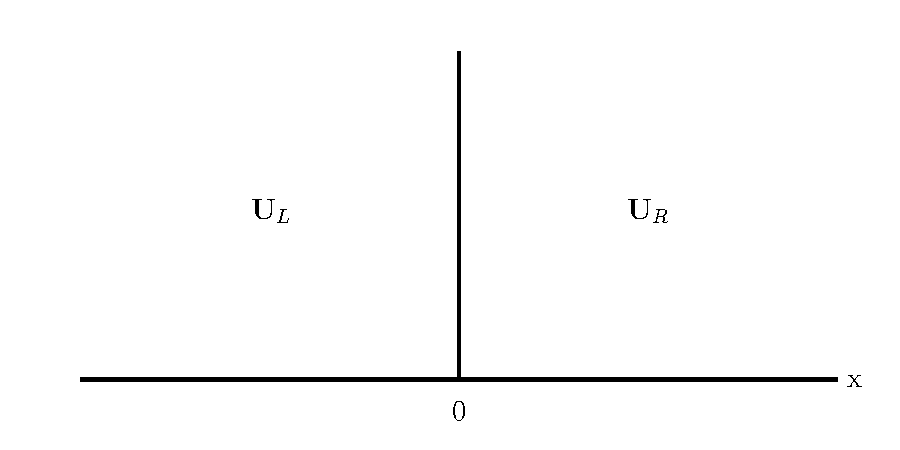
\includegraphics{./figures/riemann_problem.pdf}%
	\caption{
		The Riemann Initial Value Problem in 1D.
		\label{fig:riemann-problem}
	}
\end{figure}





Unfortunately, there is no exact closed-form solution to the Riemann problem for the Euler equations.
However, it is possible to devise iterative schemes whereby the solution can be computed numerically.
To solve full fluid dynamics problems, this calculation needs to be repeated many many times, making the solution quite expensive.
For that reason, people have developed approximate Riemann solvers, which we also will have a look at.



For a full derivation of how to solve the Riemann problem for the Euler equations, see e.g. \cite{toro}.
For our purposes, it suffices to accept that (assuming we have no vacuum) as time progresses, three waves will form which will separate the two initial states $\U_L$ and $\U_R$.
This results in two new states, $\U_L^*$ and $\U_R^*$ between the initial states, because  $\U_L^*$ and $\U_R^*$ themselves will be separated by a wave.
This is shown in figure \ref{fig:riemann-solution}


\begin{figure}[H]
	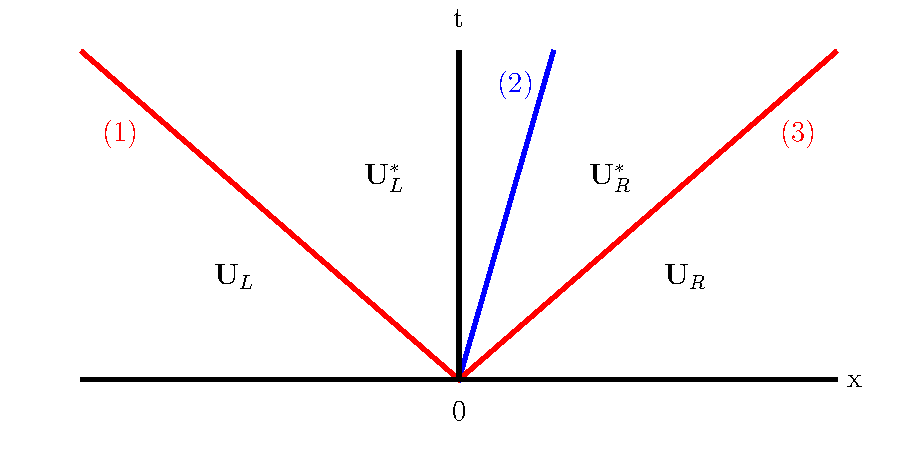
\includegraphics{./figures/riemann_solution.pdf}%
	\caption{
		The solution to the Riemann problem for Euler equations: 
		Three waves, (1), (2), and (3), arise from the origin as time evolves.
		(2) is always a contact wave, (1) and (3) can be either rarefaction or shock waves in each case, depending on the initial conditions.\\
		The initial states $\U_L$ and $\U_R$ are separated through the waves (1) and (3) from the two new arising ``star states'' $\U_L^*$ and $\U_R^*$, which themselves are separated by the contact wave (2).
		\label{fig:riemann-solution}
	}
\end{figure}












%===========================================
\subsection{Wave types and relations}
%===========================================





It turns out that we get three types of waves: A contact wave, a shock wave, and a rarefaction wave.
The middle wave is always a contact wave.
The left and right waves can be any combination of shock and/or rarefaction wave, depending on the initial conditions.
A model problem containing all three waves is shown in figure \ref{fig:riemann-solved}.
These are the wave properties:






%===========================================
\subsubsection{Contact wave}
%===========================================

The contact wave is a jump discontinuity in the density $\rho$ only.
Pressure and velocity remain constant across the contact wave.
This gives us the relations


\begin{align*}
	p^*_L &= p^*_R = p^*\\
	u^*_L &= u^*_R = u^*\\
\end{align*}

for this reason, the star state pressure and velocity will have no index indicating whether they are the left or right star state, and will be referred to as $p^*$ and $u^*$, respectively.









%===========================================
\subsubsection{Shock wave}
%===========================================

All three primitive variables $\rho$, $p$, and $u$ change across a shock wave.
A shock wave is a jump discontinuity too.
If the \textbf{leftmost} wave (wave (1) in fig. \ref{fig:riemann-solution}) is a shock wave, we have

\begin{align*}
	\rho^*_L &= 
		\frac{\frac{p^*}{p_L} + \frac{\gamma - 1}{\gamma+1}}{\frac{\gamma - 1}{\gamma+1} \frac{p^*}{p_L} + 1} \rho_L \\
	u^* &= 
		u_L - \frac{p^* - p_L}{\sqrt{\frac{p^* + B_L}{A_L}}}\\
		& = u_L - f_L(p^*) \\
	A_L &= 
		\frac{2}{(\gamma + 1) \rho_L}\\
	B_L &= 
		\frac{\gamma - 1}{\gamma + 1} p_L
\end{align*}

$f_{L}$ is given in eq. \ref{eq:riemann-pstar}, and the shock speed is
\begin{align*}
	S_L = u_L - a_L \left[\frac{\gamma + 1}{2 \gamma} \frac{p^*}{p_L} + \frac{\gamma - 1}{2\gamma} \right]^{\half}
\end{align*}

where $a_L$ is the sound speed in the left state $U_L$.



For a \textbf{right shock wave}, i.e. when wave (3) is a shock wave, we have the relations


\begin{align*}
	\rho^*_R &= 
		\frac{\frac{p^*}{p_R} + \frac{\gamma - 1}{\gamma+1}}{\frac{\gamma - 1}{\gamma+1} \frac{p^*}{p_R} + 1} \rho_R \\
	u^* &= 
		u_R + \frac{p^* - p_R}{\sqrt{\frac{p^* + B_R}{A_R}}}\\
		& = u_R + f_R(p^*) \\
	A_R &= 
		\frac{2}{(\gamma + 1) \rho_R}\\
	B_R &= 
		\frac{\gamma - 1}{\gamma + 1} p_R
\end{align*}

and the shock speed is
\begin{align*}
	S_R = u_R + a_R \left[\frac{\gamma + 1}{2 \gamma} \frac{p^*}{p_R} + \frac{\gamma - 1}{2\gamma} \right]^{\half}
\end{align*}

where $a_R$ is the sound speed in the left state $U_L$. $f_R$ is given in equation \ref{eq:riemann-pstar}.


\todo{check $u^*$: is + $B_R$ correct?\\ actually, check all equations }








%===========================================
\subsubsection{Rarefaction wave}
%===========================================

Rarefaction waves are smooth transitions, not infinitesimally thin jump discontinuities.
This makes them really easy to spot in the solutions of Riemann problems, see fig. \ref{fig:riemann-solved}.
Across rarefactions, entropy is conserved.

The rarefaction waves are enclosed by the head and the tail of the wave, between which we have a smooth transition which is called the ``fan''.
The head is the ``front'' of the wave, i.e. the part of the wave that gets furthest away from the origin as time progresses.
The tail is the ``back'' of the wave, i.e. the part of the wave that stays closest to the origin as time progresses.
The wave speeds of the head, $S_H$, and of the tail, $S_T$, are both given below.


If we have a \textbf{left-facing} rarefaction, i.e. if wave (1) is a rarefaction wave, we have

\begin{align*}
	\rho^*_L &= 
		\rho_L \left( \frac{p^*}{p_L} \right) ^ \frac{1}{\gamma}\\
	u^* &= 
		u_L - \frac{2 a_L}{\gamma - 1} \left[ \left( \frac{p^*}{p_L} \right) ^ \frac{\gamma - 1}{2 \gamma} -1  \right]\\
		& = u_L - f_L(p^*) \\
\end{align*}

$f_{L}$ is given in eq. \ref{eq:riemann-pstar}, and $a_L$ is the sound speed in the left state $U_L$.


The wave speeds of the head, $S_H$, and the tail, $S_T$, for the left facing wave are
\begin{align*}
	S_{HL} &= u_L - a_L\\
	S_{TL} &= u^* - a^*_L\\
	a^*_L  &= a_L \left( \frac{p^*}{p_L} \right) ^ \frac{\gamma - 1}{2 \gamma}
\end{align*}


Finally, the solution inside the rarefaction fan, i.e. in regions where $S_{HL} \leq \frac{x}{t} \leq S_{TL}$, is 

\begin{align*}
	\rho_{\text{fan}, L} &= 
		\rho_L \left[ \frac{2}{\gamma + 1} + \frac{\gamma - 1}{\gamma + 1} \frac{1}{a_L} \left(u_L - \frac{x}{t}\right) \right] ^ \frac{2}{\gamma -1 }\\
	u_{\text{fan}, L} &= 
		\frac{2}{\gamma + 1} \left[ \frac{\gamma - 1}{2} u_L + a_L + \frac{x}{t}  \right] \\
	p_{\text{fan}, L} &= 
		p_L \left[ \frac{2}{\gamma + 1} + \frac{\gamma - 1}{\gamma + 1} \frac{1}{a_L} \left(u_L - \frac{x}{t}\right) \right] ^ \frac{2 \gamma}{\gamma -1}
\end{align*}









If we have a \textbf{right-facing rarefaction}, i.e. if wave (1) is a rarefaction wave, we have

\begin{align*}
	\rho^*_R &= 
		\rho_R \left( \frac{p^*}{p_R} \right) ^ \frac{1}{\gamma}\\
	u^* &= 
		u_R - \frac{2 a_R}{\gamma - 1} \left[ 1 - \left( \frac{p^*}{p_R} \right) ^ \frac{\gamma - 1}{2 \gamma}  \right]\\
		&= u_R + f_R(p^*)
\end{align*}

where $a_R$ is the sound speed in the left state $U_R$.
$f_R$ is given in equation \ref{eq:riemann-pstar}.





The wave speeds of the head, $S_H$, and the tail, $S_T$, for the left facing wave are
\begin{align*}
	S_{HR} &= u_R + a_R\\
	S_{TR} &= u^* + a^*_R\\
	a^*_R  &= a_R \left( \frac{p^*}{p_R} \right) ^ \frac{\gamma - 1}{2 \gamma}
\end{align*}




Finally, the solution inside the rarefaction fan, i.e. in regions where $S_{HL} \leq \frac{x}{t} \leq S_{TL}$, is 

\begin{align*}
	\rho_{\text{fan}, R} &= 
		\rho_R \left[ \frac{2}{\gamma + 1} - \frac{\gamma - 1}{\gamma + 1} \frac{1}{a_R} \left(u_R - \frac{x}{t}\right) \right] ^ \frac{2}{\gamma -1 }\\
	u_{\text{fan}, R} &= 
		\frac{2}{\gamma + 1} \left[ \frac{\gamma - 1}{2} u_R - a_R + \frac{x}{t}  \right] \\
	p_{\text{fan}, R} &= 
		p_R \left[ \frac{2}{\gamma + 1} - \frac{\gamma - 1}{\gamma + 1} \frac{1}{a_R} \left(u_R - \frac{x}{t}\right) \right] ^ \frac{2 \gamma}{\gamma -1}
\end{align*}












%===========================================
\subsubsection{Which wave type do we have?}
%===========================================


As written before, the middle wave (wave (2) in fig. \ref{fig:riemann-solution} ) is always a contact wave, while the other two waves are any combination of rarefaction and/or shock wave.
It turns out that the condition for a rarefaction or shock wave is remarkably simple.

For the left wave (wave (1)):

\begin{align}
	p^* > p_L: && &\quad \text{ (1) is a shock wave}\\
	p^* \leq p_L: && &\quad \text{ (1) is a rarefaction wave}
\end{align}

and for the right wave (wave (3)):

\begin{align}
	p^* > p_R: && & \quad \text{ (3) is a shock wave} \\
	p^* \leq p_R: && & \quad \text{ (3) is a rarefaction wave} 
\end{align}

See \cite{toro} for more details.










%===========================================
\subsubsection{Solution for $p^*$}
%===========================================

The only thing missing to have a complete solution to the Riemann problem for the Euler equations is an expression how to obtain $p^*$, the pressure in the star region, depending on the initial conditions $U_L$ and $U_R$.
We make use of the fact that $p^*$ and $u^*$ are constant across the star region to relate $U_L$ and $U_R$, or more precisely the primitive states $\mathbf{W}_L$ and $\mathbf{W}_R$ which can easily be derived from the conservative ones.
For both shock and rarefaction waves on either side, we have equations for $u^*$ depending on the outer states  $\mathbf{W}_L$ and $\mathbf{W}_R$ and $p^*$.
By setting $u^*_L - u^*_R = 0$, which must hold, we get the equation

\begin{align}
	f(p, \mathbf{W}_L, \mathbf{W}_R) \equiv f_L(p, \mathbf{W}_L) + f_R(p, \mathbf{W}_R) + (u_R - u_L) = 0
\end{align}

with 

\begin{align}
	f_{L,R} &= 
		\begin{cases}
			(p - p_{L,R}) \left[ \frac{A_{L,R}}{p + B_{L,R}} \right]^{\frac{1}{2}}
				& ~\text{ if } ~ p > p_{L,R} ~ \quad \text{(shock)} \\
			\frac{2 a_{L,R}}{\gamma - 1} \left[ \left( \frac{p}{p_{L,R}} \right)^ \frac{\gamma -1}{2 \gamma} - 1 \right]
				& ~\text{ if } ~ p \leq p_{L,R} ~ \quad \text{(rarefaction)} \label{eq:riemann-pstar}\\
		\end{cases} \\
	A_{L,R} &= 
		\frac{2}{(\gamma + 1) \rho_{L,R}}\\
	B_{L,R} &= 
		\frac{\gamma - 1}{\gamma + 1} p_{L,R}
\end{align}











\todo{add image of riemann solution with all three wave types. Label it fig:riemann-solved}


















%====================================================================
\subsection{Exact Solver}
%====================================================================


The equation for the pressure in the star region \ref{eq:riemann-pstar} can't be solved analytically, but it can be solved iteratively.

Since we have the analytic function and the first derivative w.r.t. $p$ can be computed, i.e.

\begin{align*}
	\frac{\del f_{L,R}}{\del p} &= 
		\begin{cases}
			\left[ \frac{A_{L,R}}{p + B_{L,R}} \right]^{\frac{1}{2}} \left( 1 - \frac{1}{2} \frac{p - p_{L,R}}{p + B_{L,R}} \right) 
				& ~\text{ if } ~ p > p_{L,R} ~ \quad \text{(shock)} \\
			\frac{a_{L,R}}{\gamma p_{L,R}}  \left( \frac{p}{p_{L,R}} \right)^ \frac{-(\gamma+1)}{2 \gamma}
				& ~\text{ if } ~ p \leq p_{L,R} ~ \quad \text{(rarefaction)} \label{eq:riemann-pstar-dp}\\
		\end{cases} \\
	A_{L,R} &= 
		\frac{2}{(\gamma + 1) \rho_{L,R}}\\
	B_{L,R} &= 
		\frac{\gamma - 1}{\gamma + 1} p_{L,R}
\end{align*}


Then, using the Newton-Raphson iteration, we can find the solution using the prescription

\begin{align}
	p_{n+1} = p_n - \frac{f(p_n)}{\frac{\del f(p_n)}{\del p}}
\end{align}


we re-iterate until it converges, i.e. when the relative pressure change 

\begin{align}
	\frac{|p_k - p_{k+1}|}{\frac{1}{2} | p_k + p_(k+1) | } < \epsilon
\end{align}

where $\epsilon$ is some tolerance. Default value is set in \texttt{defines.h} as \verb|#define EPSILON_ITER 1e-6|.


We need to find a first guess for the pressure. 
An ok way to do it is to take the average:
\begin{align*}
	p_0^* = \frac{1}{2} (p_L + p_R)
\end{align*}

The implemented way is based on a linearised solution based on primitive variables:
\begin{align*}
	p_{PV} &= \frac{1}{2} (p_L + p_R) - \frac{1}{8} (u_R - u_L)(\rho_L + \rho_R)(a_L + a_R)\\
	p_0^* &= \max(\epsilon, p_{PV})
\end{align*}

Note that every step along the iteration, we must make sure that we didn't accidentally get negative pressures, and limit it to zero (or the tolerance $\epsilon$). 
If it drops below zero, it might get stuck there, and then all hell breaks loose.
(Seriously, you will get NANs because you're trying to take fractal powers of negative stuff.)


And that's it for the exact solver.
All that is left to do is sample the solution, which is described in section \ref{chap:sampling-solution}.






%====================================================================
\subsection{Approximate Solvers}
%====================================================================



%====================================================================
\subsubsection{HLL Solver}
%====================================================================


%====================================================================
\subsubsection{HLLC Solver}
%====================================================================


%====================================================================
\subsubsection{Two-Rarefaction Riemann Solver (TRRS)}
%====================================================================


%====================================================================
\subsubsection{Two-Shock Riemann Solver (TSRS)}
%====================================================================














%====================================================================
\subsection{Dealing with Vacuum}
%====================================================================


Vacuum is characterized by the condition $\rho = 0$.
With out equation of state, we also have $p = 0$ and $E = 0$ following from $\rho = 0$.
The structure of the solution to the Riemann problem is different, there is no more star region.
It can be shown that a shock wave can't be adjacent to a vacuum.
Instead, we have a rarefaction wave and a contact wave which coalesces with the tail of the rarefaction.
So we have a jump discontinuity next to the vacuum, which makes perfect sense, and this discontinuity will travel with some ``escape velocity'' $u_{vac}$.
Hence it makes sense to characterize the vacuum state as $\mathbf{W}_{vac} = (0, u_0, 0)$.

There are three cases to consider:


\begin{enumerate}

	\item \textbf{The right state is a vacuum:}
	
		The vacuum front travels with the velocity
		\begin{equation}
			S_{vac, L} = u_L + \frac{2 a_L}{\gamma - 1}
		\end{equation}
		and left of it we have a left going rarefaction wave, i.e.
		\begin{align}
			\mathbf{W}_{L, \text{ with vacuum }} = 
				\begin{cases}
					\mathbf{W_L} & \quad \text{ if } \frac{x}{t} \leq u_L - a_L \\
					\mathbf{W_{L, \text{inside fan}}} & \quad \text{ if } u_L - a_L < \frac{x}{t} < S_{vac, L} \\
					\mathbf{W_{vac}} & \quad \text{ if } \frac{x}{t} \geq S_{vac, L}\\
				\end{cases}
		\end{align}
		
	\item \textbf{The left state is a vacuum:}
	
		The vacuum front travels with the velocity
		\begin{equation}
			S_{vac, R} = u_R - \frac{2 a_R}{\gamma - 1}
		\end{equation}
		and right of it we have a right going rarefaction wave, i.e.
		\begin{align}
			\mathbf{W}_{R, \text{ with vacuum }} = 
				\begin{cases}
					\mathbf{W_{vac}} & \quad \text{ if } \frac{x}{t} \leq S_{vac, R}\\
					\mathbf{W_{R, \text{inside fan}}} & \quad \text{ if } S_{vac, R} < \frac{x}{t} <   u_R + a_R\\
					\mathbf{W_R} & \quad \text{ if } \frac{x}{t} \geq u_R + a_R \\
				\end{cases}
		\end{align}
		
	\item \textbf{ Vacuum is being generated }
	
		In certain cases, with both the left and the right state being non-vacuum states, vacuum can be generated in regions of the solution.
		Just think what might happen if the left state has high velocity towards the left, and the right state having a high velocity towards the right, leaving the center region empty.
		The result is that we have a vacuum state emerging around the center, bounded by two vacuum fronts $S_{vac, L}$ on the left side and $S_{vac, R}$ on the right side.
		The full solution is
		\begin{align}
			\mathbf{W} = 
				\begin{cases}
					\mathbf{W}_{L, \text{ with vacuum }} & \quad \text{ if } \frac{x}{t} \leq S_{vac, L}\\
					\mathbf{W}_{vac} & \quad \text{ if } S_{vac, L} < \frac{x}{t} <  S_{vac, R}\\
					\mathbf{W}_{R, \text{ with vacuum }} & \quad \text{ if } \frac{x}{t} \geq S_{vac, R} \\
				\end{cases}
		\end{align}
		
		
		When do we have a vacuum generating condition?
		Well, $S_{vac, L} \leq S_{vac, R}$ must hold, hence
		\begin{align}
			\Delta u_{crit} \equiv \frac{2 a_L}{\gamma - 1 } + \frac{2 a_R}{\gamma - 1 } \leq u_R - u_L
		\end{align}

\end{enumerate}













%====================================================================
\subsection{Sampling the Solution}\label{chap:sampling-solution}
%====================================================================

With the solvers readily available, the final task is to sample the solution at some given point $(x, t)$.
Assuming we have computed all the star region state variables, what is left to do is to determine in which case the point $(x, t)$ is located.
The flow chart of decision making and finally which relations to use is shown in figure \ref{fig:sampling-solution}.


\begin{sidewaysfigure}
	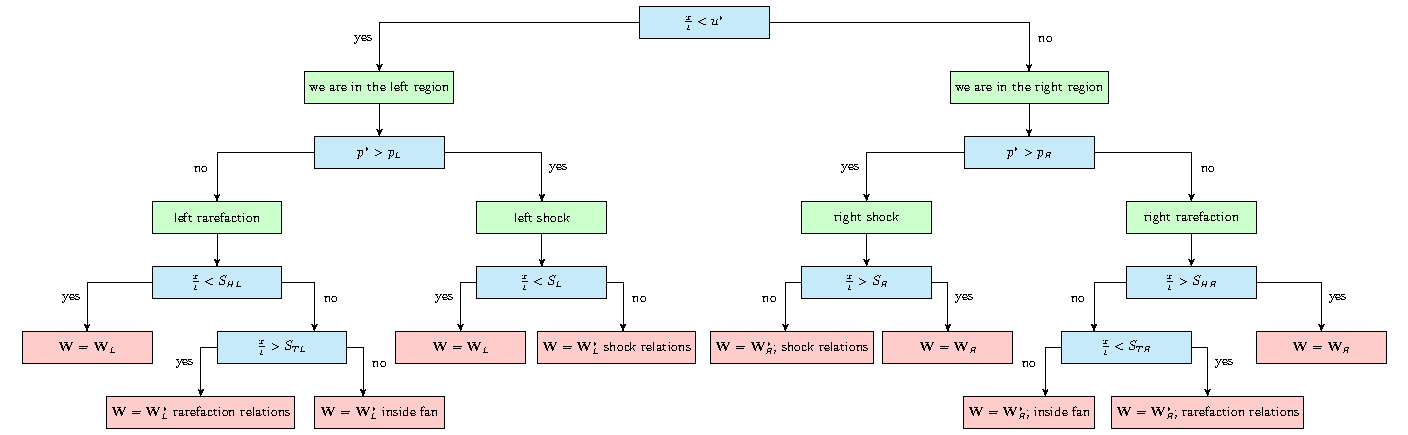
\includegraphics[]{./figures/tikz/sampling_the_solution.pdf}%
	\caption{Flow chart to sample the solution of the Riemann problem for the Euler equations at a given point $(x, t)$.
		\label{fig:sampling-solution}
	}
\end{sidewaysfigure}

Initially all we need to compute is the star states, then we sample the solution at the given point that we're interested in, and the flowchart will tell us which states we need to compute using which relations.
